
In this section we present our study results by answering our research questions. For each question, we discuss the motivation behind it, the approach to answering it and finally the results obtained.

\begin{table*}
	\caption{Summary of metrics}
	\label{tab:bla}
	\centering{}%
	\begin{tabular}{|c|c|c|c|c|c|c|c|}
		\hline 
		\multirow{2}{*}{Projects} & \multirow{2}{*}{Metrics} & \multicolumn{3}{c|}{Non-Bug fixing Commits} & \multicolumn{3}{c|}{Non-Bug fixing Commits}\tabularnewline
		\cline{3-8} 
		&  & Min Value & Max Value & Mean Value & Min Value & Max Value & Mean Value\tabularnewline
		\hline 
		\multirow{3}{*}{Hadoop} & New Logs & 0 & 184 & 0.245 & 0 & 197 & 0.533\tabularnewline
		\cline{2-8} 
		& Removed Logs & 0 & 33 & 0.093 & 0 & 143 & 0.175\tabularnewline
		\cline{2-8} 
		& Modified Logs & 0 & 67 & 0.124 & 0 & 83 & 0.227\tabularnewline
		\hline 
		\multirow{3}{*}{Hbase} & New Logs & 0 & 211 & 0.309 & 0 & 534 & 0.718\tabularnewline
		\cline{2-8} 
		& Removed Logs & 0 & 49 & 0.147 & 0 & 233 & 0.281\tabularnewline
		\cline{2-8} 
		& Modified Logs & 0 & 71 & 0.209 & 0 & 187 & 0.271\tabularnewline
		\hline 
		\multirow{3}{*}{Qpid} & New Logs & 0 & 87 & 0.116 & 0 & 477 & 0.796\tabularnewline
		\cline{2-8} 
		& Removed Logs & 0 & 23 & 0.046 & 0 & 97 & 0.270\tabularnewline
		\cline{2-8} 
		& Modified Logs & 0 & 72 & 0.084 & 0 & 125 & 0.343\tabularnewline
		\hline 
	\end{tabular}
\end{table*}



\begin{table*}[t]
	\caption{P values and Effect Size of for comparison	. A positive effect size means bug fixing commits are larger. P-values are bold if it is less than 0.05.}
	\label{tab:logchange}
	\centering{}%
	\begin{tabular}{|>{\centering}m{4.1cm}|>{\centering}m{1.5cm}|c|>{\centering}p{1.5cm}|c|>{\centering}p{1.5cm}|c|}
		\hline 
		Projects & \multicolumn{2}{c|}{Hadoop} & \multicolumn{2}{c|}{Hbase} & \multicolumn{2}{c|}{Qpid}\tabularnewline
		\hline 
		Metrics & P-Values & Effect Size & P-Values & Effect Size & P-Values & Effect Size\tabularnewline
		\hline 
		Modified Log Churn  & \textbf{2.88e-4} & 0.167(small) & \textbf{0.0353} & 0.0886 & \textbf{0.0281} & 0.329(small)\tabularnewline
		\hline 
		New Log Churn & \textbf{0.00202} & 0.0078 & \textbf{0.00353} & 0.134 & \textbf{0.0032} & 0.234(small)\tabularnewline
		\hline 
		Deleted Log Churn & 0.087 & -0.0455 & \textbf{0.00489} & 0.120 & \textbf{0.00952} & 0.042\tabularnewline
		\hline 
	\end{tabular}
	
\end{table*}



\subsection*{\textbf{RQ1: Are logs leveraged more during bug fixes? }}


\subsubsection*{\textbf{Motivation}}

Prior research has shown that logs are used during bug fixing~\cite{EMSEIAN}. During debugging, developers update log statements, to gain more run-time information of the systems and ensure that future occurrences of a similar bug can be resolved easily with the updated information. 
However, to the best of our knowledge, there exists no large scale empirical study to show how extensively logs are leveraged during bug fixes. Moreover, little is known about how bugs are leveraged during bug fixes. 


% But, this is not
%the only reason for using logging in a system. So in our first research
%question we try to address this issue. Answering this questions helps
%us understand where developers log more.


\subsubsection*{\textbf{Approach}}

%Its intuitive that logs are generally modified when bugs are fixed.
%This is because prior research has already proved that a module
%that has been modified continually, has higher chance
%of having bugs than modules which have not been modified \cite{Khosh}.
%So,
We try to find if there is a difference between bug fixing and non-bug fixing commits with respect to log churn. To do this, we used the data sets obtained in previous section i.e modified, new and removed logs, and we calculated code churn for each data set. We used the total code churn of a revision to control the other metrics. The 3 new metrics are:
\begin{equation}
Modified\ log\ churn\ ratio = \frac{\#\ modified\ log}{total\ code\ churn } 
\label{eq1}
\end{equation}
\begin{equation}
New\ log\ churn\ ratio = \frac{\#\ new\ log}{total\ code\ churn } 
\label{eq2}
\end{equation}
\begin{equation}
Removed\ log\ churn\ ratio = \frac{\#\ removed\ log\ churn}{total\ code\ churn }
\label{eq3} 
\end{equation}

To determine whether there is a statistically significant difference for these metrics, in bug-fixing and non-bug-fixing commits, we perform the \textsl{MannWhitney U test} (Wilcoxon rank-sum test)~\cite{gehan1965generalized}. We choose {\em MannWhitney U test} because we our metrics are highly skewed (shown in table~\ref{tab:bla}) and as it is a non-parametric test, which does not have any assumptions about the distribution of the sample population. A p-value of \ensuremath{\le} 0.05 means that the difference between the two data sets is statistically significant and we may reject the null hypothesis (i.e., there is no statistically significant difference of our metrics in in bug-fixing and non-bug-fixing commits). By rejecting the null hypothesis, we can accept the alternative hypothesis, which tells us there is statistically significantly difference of our metrics in bug-fixing and non-bug-fixing commits.

%and if we use standard T-test the
%resulting p-value will be wrong. {\em Wilcoxon test} is a non-parametric
%test, meaning the distribution of the population does not factor into
%the results.

We also use {\em effect sizes} to measure how big is the difference of our metrics ($modified\ log\ churn\ ratio$, $new\ log\ churn\ ratio$, and $removed\ log\ churn\ ratio$) between the bug fixing and non-bug-fixing commits. Unlike {\em MannWhitney U test}, which only tells us whether the difference between the two distributions are statistically significant, effect sizes quantify the difference between two distributions. Researchers have shown that reporting only the statistical significance may lead to erroneous results  (i.e., if the sample size is very large, p-value can be small even if the difference is trivial). We use {\em Cohen's d} to quantify the effects. {\em Cohen's d} measures the effect size statistically, and has been used in prior engineering studies. {\em Cohen's d} is defined as:
\begin{equation} \text{{\em Cohen's d}} = \frac{\bar{x}_1 - \bar{x}_2}{s},
\label{eq:cohensd}
\end{equation}
where $\bar{x}_1$ and $\bar{x}_2$ are the mean of two populations, and $s$ is the pooled standard deviation \cite{HartungBook2011}. As software re-engineering has different thresholds for 
{\em Cohen's d} \cite{Effectsize}, the new scale is shown below. \\ \\
$Effect\: Size\,=\begin{cases}
0.16\,\,< & Trivial\\
0.16-0.6 & Small\\
0.6-1.4 & Medium\\
1.4\;\,\,> & Large
\end{cases}$

To understand how logs are leveraged during bug fixes, we performed a manual analysis on the modified logging statements to identify the different types of log modifications. We first collected all the commits which had logging statement changes in our projects. We selected a random sample of x commits from all the commits with logging statement changes. The size of our random sample achieves 95\% confidence level and 5\% confidence interval. We followed an iterative process, as prior research~\cite{Seaman}, to identify the different types of logging modifications, until we cannot find any new types of modifications. 

After we identify the types of log modifications, we created an automated tool to label log modifications into the four categories. We calculated the number of each type of log modifications in each commit and used {\em total code churn } as the controlling measure similar to equation~\ref{eq1} to \ref{eq3}. We used {\em MannWhitney U test} to find out whether the difference of each type of log modifications between bug fixing and non-bug fixing commits is statistically significant. We consider only those commits with log churn in this test. We also use {\em Cohen's d}, to measure how big is the difference for each type of log modification between bug fixing and non-bug fixing commits.



\subsubsection*{\textbf{Results}}


\textbf{Developers may add new logs more during bug fixes.} From table~\ref{tab:logchange}, $new\ log\ churn\ ratio$ in bug-fixing commits is statistically significantly larger than non-bug-fixing commits in all subject systems but only Qpid has non-trivial effect size. This implies in some cases developers need to add more logging statements in some places in the source code. For new projects like Qpid, some important source code is not well logged. Therefore, developers may find that they need to add logging statements to assist in bug fixing. For mature projects such as Hadoop and Hbase, source code is well logged so, developers may focus more on improving existing logging statements rather than adding new logging statements.

% completely ignore
%logging during initial development and have to spend more time starting
%from scratch. This is an extra effort which can be avoided by good
%logging practices.

\textbf{Developers do not delete logs during bug fixes.} We find that although $removed\ log\ churn\ ratio$ in bug-fixing commits is statistically significantly larger than non-bug-fixing commits in Hbase and Qpid, the effect sizes are trivial (see table~\ref{tab:logchange}). Developers do not remove logging statements for fixing bugs. In Hadoop, we find logging statements are even removed more from non-bug fixing commits than bug fixing commits. Such results confirm the findings from prior research that deleted logs do not have a strong relationship with code quality~\cite{WCSEIan}. 


\begin{table}[thb]
	\caption{Distribution of four types of log modifications.}	
	\label{tab:dist}
	\centering
	\begin{tabular}{|>{\centering}p{2.2cm}|>{\centering}p{1.3cm}|>{\centering}p{1.3cm}|>{\centering}p{1.3cm}|}
		\hline 
		Projects & \multicolumn{1}{c|}{Hadoop (\%)} & \multicolumn{1}{c|}{Hbase (\%)} & \multicolumn{1}{c|}{Qpid (\%)}\tabularnewline
		\hline 
		Relocating  & 82.6 & 61.4 & 55.8\tabularnewline
		\hline 
		Text Modification & 7.85 & 12.1 & 18\tabularnewline
		\hline 
		Variable Modification & 7.9 & 8.4 & 12.5\tabularnewline
		\hline 
		Logging Level Change & 3.85 & 5.4 & 13.6\tabularnewline
		\hline 
	\end{tabular}
\end{table}


\textbf{Logs are modified more in bug fixing commits than non-bug-fixing commits}. Table~\ref{tab:logchange} shows that $modified\ log\ churn\ ratio$ is statistically significantly higher for all subject systems and the effect sizes are non-trivial in Qpid and Hadoop. Such results show that developers often change the information provided by logging statements to assist in bug fixing. Prior research that 36\% of log messages are modified at-least once as after-thoughts~\cite{Characterizinglogs}. Developers may find out that they need different information from logs to help them fix bugs. We find that the significancy and effect size of $modified\ log\ churn\ ratio$ is bigger than $new\ log\ churn\ ratio$, which implies that developers do not tend to provide additional information in logs but rather improve the existing logs. Prior research shows that too much information provided by logs may have become a challenge for developers to fix bugs~\cite{Yuan:2014:STP:2685048.2685068}. Such finding may explain the reason why developer choose modifying logs over adding new logs.

From our manual analysis, we identified four types of log modifications. The distribution of the four types is shown in table~\ref{tab:dist}. The four types of changes are described below:

\begin{enumerate}
	\item \textbf{Log relocation.} The logging statement is kept intact with only white space changes but moved to a different place in the file.
	\item \textbf{Text modification.} The text printed from the logging statements is modified.
	\item \textbf{Variable change.} One or more variables in the logging statements are changed (added, deleted or modified).
	\item \textbf{Logging level change. } The verbosity level of logging statements are changed.
\end{enumerate}
\begin{comment}
This means that in most cases the existing logging messages do not
convey all the information necessary for a bug fix. An example of this type of change is shown below:\\


+ log.trace("setConnectionURL(" +  Util.maskUrlForLog\\(connectionURL)  ")");

- log.trace("setConnectionURL(" + connectionURL + ")");
\hypobox{- Logger.warn( `` Sample Text Goes Here '' + printAVariable );\\
+ Logger.warn( ``\textcolor{magenta}{{} New} Sample Text Goes Here
'' + printAVariable);}



% Its classified similar to Text Modification by changing
%the final condition.\linebreak{}
\hypobox{- Logger.warn( `` Sample Text Goes Here '' + \textcolor{black}{printAVariable}
);\\
+Logger.warn( `` Sample Text Goes Here '' + printAVariable + \textcolor{magenta}{printBVariale});
}

\noindent


\hypobox{- Logger.\textcolor{black}{warn}( `` Sample Text Goes Here '' +
printAVariable );\\
+ Logger.\textcolor{magenta}{debug}(`` Sample Text Goes Here ''
+ printAVariable );}
\end{comment}







%We observed
%that this is one of the most frequent type of change done in both
%buggy and non-buggy commits from table 2. To categorize this we set
%the Levenshtein distance less than 5 \textbf{and} ratio higher than
%0.9.


%To classify this we first checked if the levenshtein distance
%is less than 5 \textbf{or} levenshtein ratio greater than 0.7. If
%this condition was met, we said the log message had similarities with
%one of the deleted logs. Then we checked if the similar part was 'message'
%or 'variable' part. If there was over 0.9 similarity with the variable
%parts but not with the text part, we concluded it was text addition
%or deletion. Because this condition overlaps 'Relocating', they
%were classified first and those logs were excluded from further classification.
%\linebreak{}




%To find this we
%checked if the levenshtein distance of the entire log message is equal
%to the levenshtein distance of the log level. If this condition was
%met, it means only the part that is changing is the level of log.


\textbf{Developers modify variables more in bug fixing commits.} We find that variable change is statistically significant more in all the subject systems and has small or medium effect sizes (see table~\ref{tab:logmod}). This implies that developers may modify the variables printed in their logging statements in order to provide useful information about the system to assist in bug fixing. To better understand how developers change variables in logging statements during bug fixing, we put the variable change into three types: variable addition, variable deletion and variable modification. From table~\ref{tab:varmod}, we see that developers modify variables statistically significantly more in all projects with has non-trivial effect sizes. This implies that developers may not know what exact information is needed when they add the logging statements into the source code. The developers may realize the need of some information and modify logging statements to print the value of needed variables. Similar findings are presented in prior research that developers often have after-thoughts on logging statements~\cite{Characterizinglogs}. Similar to the above finding that developers choose modifying logs over adding logs, developers also choose modifying variables in logging statements over adding more variables, due to the massive amounts of logs can be a burden for bug fixing.


\textbf{Developers modify text in logs more during bug fixes.} We find that text modification is statistically significant more in bug-fixing commits than non-bug-fixing commits with non-trivial effect sizes (see table~\ref{tab:logmod}). This implies that in some cases, the text description in logs are not clear and developers improve the text to understand the logs better to fix the bugs. For example, in commit 1,405,354  developers modify the logging statement to provide more information about the cause of an exception being raised. Prior research finds that there exists challenge of understating logs in practice~\cite{IanIcesm}. Our results show that developers may have encountered such challenge and try to improve the text in logs for a better bug fixing. 
%
%that developers value more in providing contextual data to an existing
%log rather than writing new logging statements. 

\textbf{We found log relocation is more in bug fixes.} From table~\ref{tab:dist}, we see that there are a large number of logging changes that only relocates logging statements the code. Table~\ref{tab:logmod} shows that such relocation happens statistically significantly more in bug-fixing changes. We manually examined such commits and find that developers often forget to leverage exception handling or using proper condition statements in the code. After fixing the bug, developers often move existing logging statements into the \emph{try/catch} blocks or after condition statements. For example, in the revision 792,522 of Hadoop, we see that the a logging statements are placed into the proper \emph{try/catch} block.

\textbf{Logging levels are not modified often during bug fixes.} We find that logging level changes only happens statistically significantly more in Hadoop project. This implies developers typically do not change log levels during bug fixes. The reason of logging level not being changed during bug fix may be that developers are able to enable all the logging statements during debugging despite of what level a logging statement has. In addition, prior research shows that developers do not have a good knowledge about how to choose a correct logging level~\cite{Characterizinglogs}. 

\begin{table*}
	\protect\caption{P-values and effect size for Log modifications. P-values are bold if they are smaller than 0.05.}
	\label{tab:logmod}
	\centering{}%
	\begin{tabular}{|>{\centering}m{5cm}|c|c|c|c|c|c|}
		\hline 
		\multicolumn{1}{|>{\centering}p{4cm}|}{Projects} & \multicolumn{2}{c|}{Hadoop} & \multicolumn{2}{c|}{Hbase} & \multicolumn{2}{c|}{Qpid}\tabularnewline
		\hline 
		Metrics & P-values  & Effect Size & P-values  & Effect Size & P-values  & Effect Size\tabularnewline
		\hline 
		Log relocation & \textbf{1.69e-11} & 0.260(small) & \textbf{6.33e-03} & 0.2092(small) & \textbf{9.14e-08} & 0.987(med)\tabularnewline
		\hline 
		Text modification & \textbf{7.75e-04} & 0.153(small) & \textbf{2.94e-05} & 0.308(small) & \textbf{4.68e-08} & 0.531(small)\tabularnewline
		\hline 
		Variable change  & \textbf{1.94e-06} & 0.447(small) & \textbf{3.51e-04} & 0.614(med) & \textbf{5.19e-05} & 1.209(med)\tabularnewline
		\hline 
		Logging level change & \textbf{0.0057} & 0.412 & 0.153 & -0.05 & 0.341 & 0.396\tabularnewline
		\hline 
	\end{tabular}
\end{table*}

\begin{table*}[tbh]
	\caption{P-values and effect size for the different types of variable change. P-values are bold if they are smaller than 0.05.}
	\label{tab:varmod}
	\centering
	\begin{tabular}{|c|c|c|c|c|c|c|}
		\hline 
		\multicolumn{1}{|>{\centering}p{2cm}|}{Projects} & \multicolumn{2}{c|}{Hadoop} & \multicolumn{2}{c|}{Hbase} & \multicolumn{2}{c|}{Qpid}\tabularnewline
		\hline Metrics & P-values  & Effect Size & P-values  & Effect Size & P-values  & Effect Size\tabularnewline
		\hline  Variable addition & 0.22  & -0.069  & 0.129 & 0.222 & 0.486 & -0.152 \\ 
		\hline  Variable deletion & 0.25 &   -0.114 & 0.585 &  0.165  & 0.22 & -0.195  \\ 
		\hline Variable modification & \textbf{0.047} &.221(small)  & \textbf{0.0032} & 0.268(small) & \textbf{1.61-05} & 0.550(small)   \\ 
		\hline 
	\end{tabular} 
\end{table*}
%\fbox{\begin{minipage}[t]{0.9\columnwidth}%
%\textbf{Finding: } Developers log more during bug fixes than other types of changes.
%
%\textbf{Implication:} Developers modify logs more during the debugging process. This implies that, developers have fair idea which
%modules can lead to bugs, so they write logging statements in those modules to assist them.
%But as these logs do not convey all the information necessary 
%so they are modified later by the developers.%
%\end{minipage}}
%
%\hphantom{}
\hypobox{Developers change logs more in bug-fixing commits than non-bug-fixing commits. In particular, developers modified logs to change the variables in logging statements during bug fixes. Such results show that developers often realize the needed information to be logged and change the printed variables in logging statement to assist in fixing bugs.}


\begin{comment}
\subsection*{\textbf{RQ2: What types of modifications to logs are more frequent during bug fix ?}}


\subsubsection*{\textbf{Motivation}}

From RQ 1 we found that logs are modified more during bug fixes. In this RQ, we want to know how logs are leveraged during bug fixes, in particular the different types of modifications to logs.

%
% However, as this information is not sufficient to understand the usefulness of logs in debugging process; in this RQ we study the different types of modifications done to logs. This will provide more information and insight into how different types logging changes assist in the debugging process.
% and also investigate how these changes assist in fixing bugs. This is an important step in 
%But the effect size was still
%small within the 0.1 - 0.3 range. So we tried to look at the different
%types of logging modifications which occur.




\subsubsection*{\textbf{Approach}}

We performed a manual analysis on the modified logging statements to identify the different types of log modifications. We first collected all the commits which had logging statement changes in our projects. We selected a 5\% random sample from all the commits with logging statement changes. We followed a iterative process \cite{Seaman} to identify the different types of logging modifications, that developers make in the source code till we cannot find any new types of modifications.
%The steps we followed were -
%\begin{itemize}
%	\item \textbf{Step 1.} Collect all the commits with log churn from both
%	data sets (i.e Buggy and Non-Buggy ), in all projects into a single data
%	set $Rev_{Total}$ 
%%	and $Non-Bug_{Total}$, 
%	\item \textbf{Step 2.} Randomly sample a subset from $Rev_{Total}$
%%	and $Non-Bug_{Total}$
%	, to get $Rev_{Subset}$ 
%%	and $Non-Bug_{Subset}$,
%	so that it has 95\% confidence level and $\pm$ 5\% confidence interval.
%	\item \textbf{Step 3.} For each commit in the data set, identify common patterns of changes which occur.   
%%	 find which category
%%	of log modification they belong to ( i.e. logging level, variable
%%%	modification, text modification or restructuring)
%	\item \textbf{Step 4.} Repeat step 3 for all the commits in the subset till
%	distribution is obtained.
%\end{itemize}
%
% From our manual analysis, we found that in our data set, changes occur either in the logging level, in the textual information or in the parameters. We identified 4 types of changes in logging level namely -\\
%\\

%To find the types of modifications in logging messages, we looked
%at the components of a log message. We observed 3 main components
%namely the log level ( Warn, Error, Debug, Trace or Fatal), the message
%part and the variables part. The changes can be made to each of these
%parts and we divided the logging changed based on these categories.
%We used Levenshtein distance \cite{levenshtein} and ratio's to filter
%the logging changes into these categories. The four categories are:




%Using {\em Levenshtein } measures , we automated the process of categorization into the four categories. This is done by parsing all the changed logging statements in each commit and comparing to the 4 categories found. We also obtained the distribution for each type of change as show in table 2.
For every commit, we found calculate the number of modifications in each category and used { \em total churn } as the controlling measure. The four metrics are- (1) Relocating log Churn, (2) Text Modification Churn, (3) Variable Modification Churn and (4) Logging Level Churn.


%\begin{enumerate}
%	\item \textbf{Relocation Churn: } 
%	As explained above we categorized all the logging statements into
%	4 types. This metric counts the total number of logs of type 'Relocating'
%	were present in each commit. 
%	\item \textbf{Text Modification Churn: } This metric is the aggregate of log changes of type 'Type Modification'	are present in each commit
%	
%	\item \textbf{Variable Modification Churn: } This metric is the aggregate of log changes of type 'Variable Modification'
%	are present in each commit.
%	\item \textbf{Logging Level Churn: } This metric is the aggregate of log changes of type 'Logging Level
%	Change' are present in each commit.
%\end{enumerate}

%do this we created smaller subsets for bug and non-buggy revisions
%which had non-zero values for each of the metrics. 
%As in section 4.1.2
%we measure the difference between the data sets through {\em Wilcoxon} tests
%and {\em Cohens.d}. 

%\subsubsection*{Relocating Churn}
%
%As explained above we categorized all the logging statements into
%4 types. This metric counts the total number of logs of type 'Relocating'
%were present in each commit. 
%
%
%\subsubsection*{Text Modification Churn}
%
%
%
%\subsubsection*{Variable Modification Churn}
%
%This metric is the aggregate of log changes of type 'Variable Modification'
%are present in each commit.
%
%
%\subsubsection*{Logging Level Churn}
%
%This metric is the aggregate of log changes of type 'Logging Level
%Change' are present in each commit.
\subsubsection*{\textbf{Results}}


%
%Another example of this 1,042,282 revision in which a log statement
%is moved from the beginning of code block to the end of block. From
%our manual study (section 5) we found that this is mostly done to
%improve the readability or increase the performance. For example in, HBASE-4288
%the logs are moved into new blocks, so they are printed only when
%'Trace/Debug' option is enabled. 

%\fbox{\begin{minipage}[]{0.85\columnwidth}%
%\textbf{Finding}: Variable modification is more significant when compared to other types of log modifications\\
%\textbf{Implication}: Developers believe adding more parameters/variables to logging statements, helps in the debugging process. This shows that logging statements evolve continually and can change multiple times across revisions.
% It also means developers can spend more time or make use of the logging tools present to log more in first commit so subsequent changes are not necessary and debugging is faster.%
%\end{minipage}}

%logging level changes are similar in both buggy and non-buggy commits.

%%From these results we have firmly established that logs are used and
%leveraged by developers during bug fixes. We also see that new logs
%are added during bug fixes than other types of changes. 


\end{comment}


\subsection*{\textbf{RQ3: Are logs useful in bug fixes?}}


\subsubsection*{\textbf{Motivation}}

In our previous research questions we found that logs are modified more frequently in bug fixes. However, we cannot come to any inference about the usefulness of logs in bug fixes. In this RQ we try  to understand the usefulness of leveraging logs during bug fixes.
% In this RQ we try to find how these changes help in the debugging process. 

%logs are in bug fixes. We also try to understand under which circumstances
%logs are helpful. We try to do this by using a measure and comparing
%our results. 


\subsubsection*{\textbf{Approach}}

To find the usefulness of logs in bug fixes we identified all JIRA issues of type 'bug' from the three subject systems. We obtained the code commits for each of these JIRA issues and identified log churn for each commit. We then split the JIRA issues into (1) bugs fixed with log changes (2) bugs fixed without log changes. We calculate the total code churn for each of the JIRA issues. We use the total code churn to measure the complexity of the issue. We then compare the total code churn of bug fixes with log changes, against bug fixes without log changes. We use \textsl{Wilcoxon} test to find the statistical significance and \textsl{Cohens.d} to measure the size of the difference. \\
%we first collected all the buggy JIRA issues for the three systems.
%Then using the churn metrics from previous step we split this buggy
%list into
% two sets - (1) bug fixes with log change (2) bug fixes
%without log change. 


We then parsed the JIRA issue files for each commit and extracted three metrics namely -

\begin{table*}[t]
\protect\caption{P-Values and Effect Size for Bug fixes}


\hphantom{}

\centering{}%
\begin{tabular}{|>{\centering}m{4.1cm}|c|c|c|c|c|c|}
\hline 
Projects & \multicolumn{2}{c|}{Hadoop} & \multicolumn{2}{c|}{Hbase} & \multicolumn{2}{c|}{Qpid}\tabularnewline
\hline 
Metrics & P -values  & Effect Size & P -values  & Effect Size & P -values  & Effect Size\tabularnewline
\hline 
Total Churn & \textbf{2.2e-16} & 0.563(small) & \textbf{2.2e-16} & 0.093 & \textbf{3.15e-08} & 0.270(small)\tabularnewline
\hline 
Resolution Time & \textbf{4.26e-03} & -0.145(small) & \textbf{7.44e-14} & -0.167(small) & 0.0865 & -0.119\tabularnewline
\hline 
\# of Comments & \textbf{2.2e-16} & -0.507(small) & \textbf{5.16e-11} & -0.289(small) & \textbf{2.34e-03} & -0.227(small)\tabularnewline
\hline 
\# of  Developers & \textbf{2.2e-16} & -0.577(small) & \textbf{2.2e-16} & -0.538(small) & \textbf{4.73e-02} & -0.375(small)\tabularnewline
\hline 
\end{tabular}
\end{table*}

\begin{enumerate}
	\item \textbf{Resolution Time:} This is the time taken from the time a bug is opened till its resolved. For example in JIRA if bug was reported in 1$ ^{st} $ Feb 2015 and
	closed in 5$ ^{th} $ Feb 2015 it means the time taken to fix the bug was 4 days.
	We used to measure  how
	long it takes for a bug to be fixed.
	
	\item \textbf {Number of Comments:} This metric gives the total number of comments are present in a JIRA
	issue. We obtained this by finding the number of comment id's present
	in the JIRA XML file. We used this measure how much effort is needed to discuss on fixing a bug.
	
	\item \textbf {Number of Developers: } Every task in JIRA is generally assigned to particular developer and
	there number of viewers who are interested in the issue and help in
	resolving it. This metric gives the number of such unique developers
	who commented on the JIRA issue posts and were involved in resolving
	it. We obtained this by finding all the unique author names in the
	XML file. We used this as a metric as it shows human effort needed.
	More number of developers involved and commenting on a issue list,
	signifies more human effort spent resolving the bug.
\end{enumerate}

%\subsubsection*{Time Taken}
%
%This is the time taken from the time a bug is opined till its resolved
%or closed. For example in JIRA if bug was reported in 01-2-15 and
%closed in 05-2-15 it means the time taken to fix the bug was 4 days.
%We used this because this is a very basic measure and tells us how
%long it takes for a bug to be fixed.
%
%
%\subsubsection*{Comments}
%
%This metric gives the total number of comments are present in a JIRA
%issue. We obtained this by finding the number of comment id's present
%in the JIRA XML file. We used this measure as it gives information
%about how complex issues are. If its a simple issue, it wont be discussed
%and will be resolved quickly. But, if its a complex bug there will
%be more discussion posts and takes longer to be resolved.
%
%
%\subsubsection*{Developers}
%
%Every task in JIRA is generally assigned to particular developer and
%there number of viewers who are interested in the issue and help in
%resolving it. This metric gives the number of such unique developers
%who commented on the JIRA issue posts and were involved in resolving
%it. We obtained this by finding all the unique author names in the
%XML file. We used this as a metric as it shows human effort needed.
%More number of developers involved and commenting on a issue list,
%signifies more human effort spent resolving the bug.

We controlled the metrics by total code churn. We used \textsl{Wilcoxon} test to measure the statistical significance of each metric in bugs fixed with log changes with bugs fixed without log changes. \textsl{Cohens.D} is used to measure the size of the difference of each metric. 

%Finally we matched this JIRA metrics without our two data segments
%based on JIRA issue numbers. The statistics of the data sets are show
%in table 5. We used \textsl{Wilcoxon} test and \textsl{Cohens.d} to measure the difference
%between the data-sets.


\subsubsection*{\textbf{Results}}

\textbf{We found that the logs are used to fix more complex bugs}. From table 7 we see that average code churn per commit is significantly higher for commits with log changes and has non-trivial effect sizes. This implies that when dealing with more complex bugs, developers may leverage logs more.

%This can be because (1) The information provided by existing logs is insufficient and hence they modify the logs to get additional data. (2) Developers are adding new methods or function and hence add logs to track the control and data flow in the new blocks.  
 
 
% From table 4, we see that in all
%projects total churn is statistically significant and has
%small effect sizes. In table 5 we again see this, where in every project
%the average churn is several magnitudes higher for bug fixing commits
%with log changes. This shows that developers always tend to change
%logs more during complex bug fixes.

%Because total churn is correlated to other metrics in our data set, we used it as our controlling measure, similar to the previous research questions. 
% measure to calculate the importance of each metric
%i.e. we take ratio of each metric against the code churn. We did this
%because in all projects logs are changed only during a complex bug
%fix. Because of this, when we measure the statistical significance
%of the 2 data sets, it will be biased. To correct this, we used 'total
%churn' as controlling measure and the results are shown in table 4.

%\begin{figure}[t]
%\includegraphics[scale=0.475]{\string"C:/Users/Suhas/Dropbox/New MSR RQ2/Hbase/Rplot01\string"}\caption
%{Cumulative Density Function of the fix time for Bug with log churn
%and Bugs without log Churn. The x-axis shows the time taken for resolution
%after its normalized using total churn. y-axis shows the cumulative
%density. }
%\end{figure}

%
%\fbox{\begin{minipage}[t]{0.9\columnwidth}%
%\textbf{Findings}: Total Churn has positive effect size
%
%\textbf{Implication}: This implies that bug fixes with log changes,
%have larger code churn. This means generally logging changes are generally
%done to more complex bugs and ignored for smaller bugs by developers. %
%\end{minipage}}
%
%\hphantom{}

\begin{figure*}
	
	\centering
	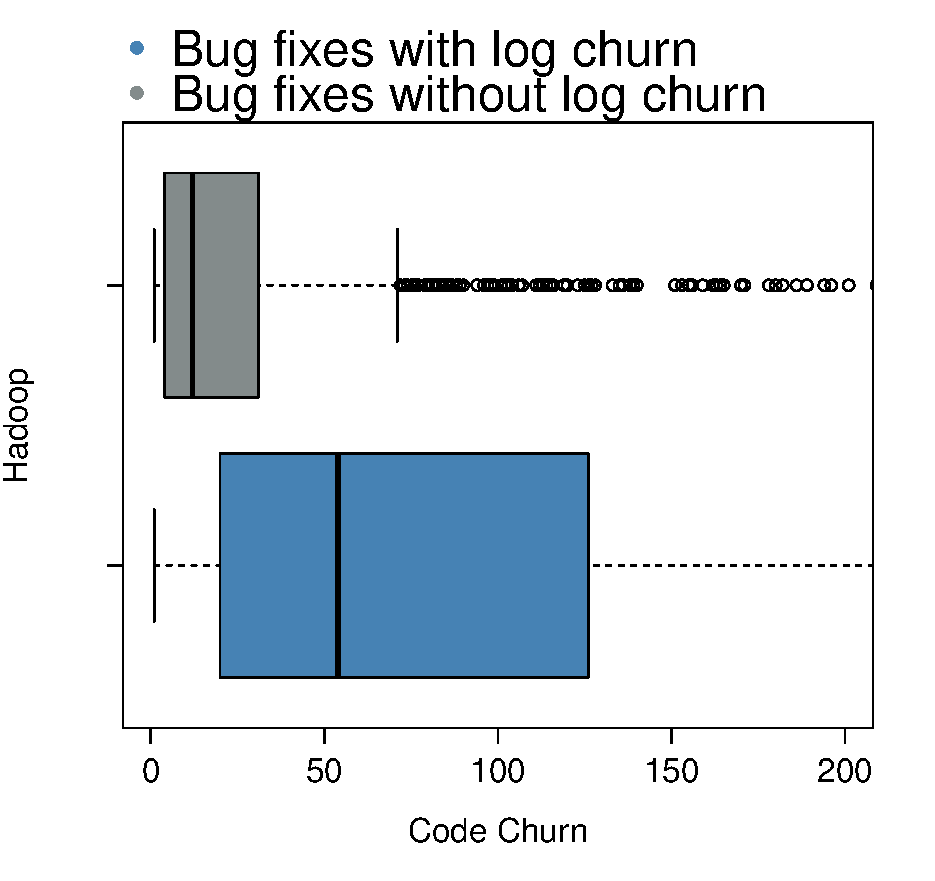
\includegraphics[width=.25\textwidth]{HadoopBoxPlot}
	\hfill
	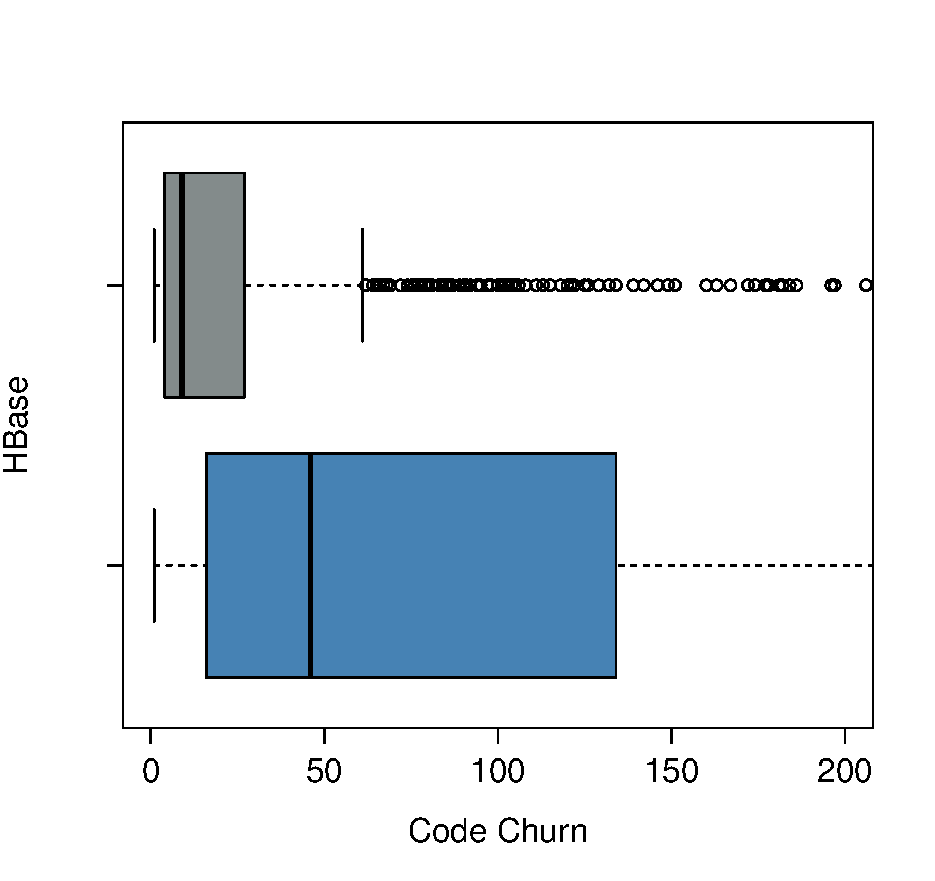
\includegraphics[width=.25\textwidth]{HBaseBoxPlot}\hfill
	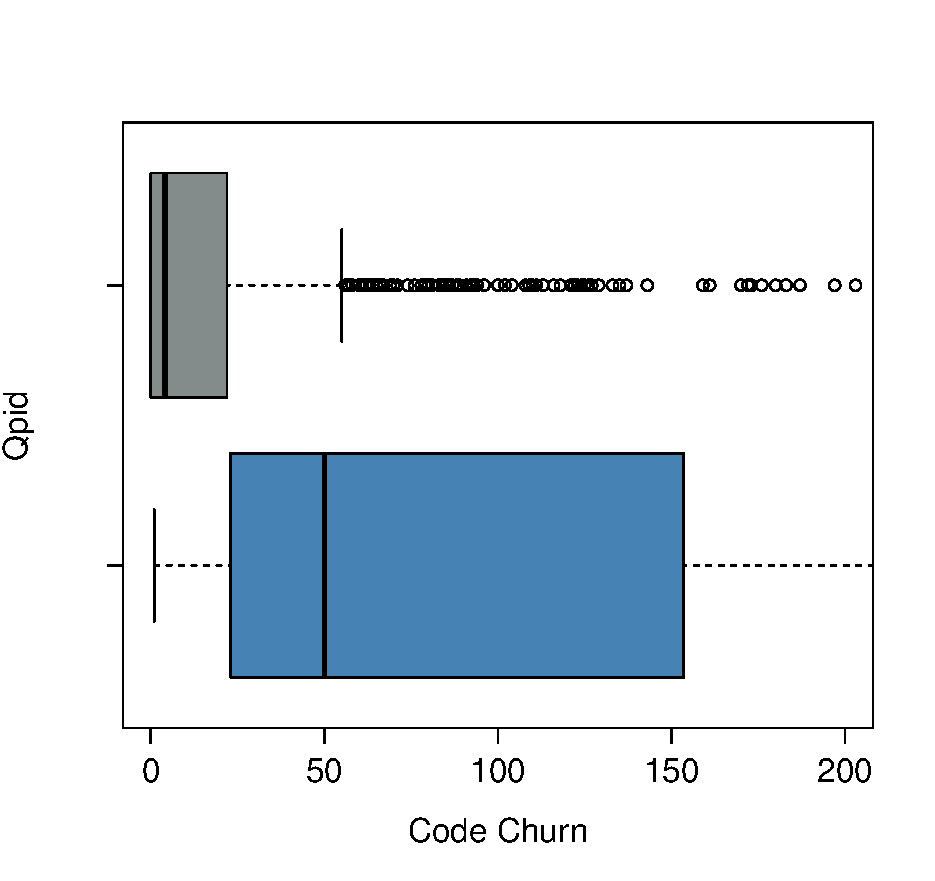
\includegraphics[width=.25\textwidth]{QpidBoxPlot}
	
	\caption{default}
	\label{fig:figure3}
	
\end{figure*}



\textbf{We found that bugs are easier to fix with logs}. After controlling the churn, we found that given two bugs of same complexity the one with log changes takes lesser time to
get resolved and needs lesser number of developers involved in the fix with less discussion. This implies that logs provide useful information for developers to discuss, diagnose and fix bugs easily. For example, logs are used in fixing issue HBASE-3074 (commit 1,005,714).
In this JIRA issue we see the very first comment is to provide additional
details in the logging message about where the connection manager
fails. When we looked at the commit, we see that the developers add
the name of the existing server which has gone stale in the logging statements. This additional data helps trace the cause of the failure and helps in the debugging process.  


%
%Because there is less developers involved in the discussion, the number of discussions posts/comments on JIRA is also less. This is because when logs are leveraged, its easier to debug the problem so resolution time is less. Developer involvement is also less because, the bug can be traced and fixed easily and long discussions about root-cause analysis is avoided. 




%This example further validates our findings
%and shows that logs are indeed very useful in the debugging process.

\hypobox{ Logs are leveraged during complex bugs and help in quicker resolution. 
	Developers leverage logging statements to fix 	complex bugs. Bug fixes with log changes are resolved quicker with fewer people and less discussions. This implies provide useful information to fix bugs.	}

%\fbox{\begin{minipage}[t]{0.9\columnwidth}%
%\textbf{Findings}: From table 4, we find all metrics have negative effect sizes and are statistically significant.
%\textbf{Implication}: 
%This implies bugs without any log churn take
%longer to be fixed, need more involvement and discussions. This shows
%that logs play a vital role in solving bug fixes. Drawing from the
%manual study done in research question two, we observed that logs
%help in locating the buggy module and when fixes are made to the module,
%developers modify the logging statements. This is cyclic process and
%hence its vital that developers log in the initial development process.%
%\end{minipage}}

\hphantom{}
%
%To validate our study we did a manual study on to understand how logs
%are actually used in the debugging process. This is explained in further
%details in the subsequent section. 
